%!TEX root = main.tex

\section{Experiments}
\label{sec:experiments}

We benchmark \DF (factorized IVM) against \IVM (first-order IVM) and \DBT (DBToaster's fully recursive higher-order IVM) on two in-database machine learning tasks: training  linear regression models and building Chow-Liu Trees over database joins under updates; and on one database task: maintaining and enumerating $q$-hierarchical join queries under updates. 

We summarize our experimental findings as follows.

(1) For maintaining covariance matrices over continuous variables, \DF outperforms \DBT and \IVM by up to three orders of magnitude. This is primarily due to the use of the covariance ring in \DF, which can capture the maintenance for an entire covariance matrix of 100-800 entries with under ten views. In contrast, \DBT requires 600-3,000 views, while \IVM needs as many delta queries as matrix entries.
A similar conclusion holds for maintaining covariance matrices over continuous and categorical variables and also only over categorical variables, albeit the performance gap becomes smaller.
Thanks to the covariance ring, \DF also has a low memory footprint, on par with \IVM and 4-16x less than \DBT.

(2) Maintaining linear regression models over the covariance matrices takes insignificant time if the batch gradient descent resumes with the values for the model parameters computed after the previous update batch.

(3) Maintaining the mutual information matrices and Chow-Liu trees over the covariance matrices requires recomputation after every update batch and this can decrease the throughput of \DF by up to one order of magnitude.

(4) For $q$-hierarchical queries,  \DF is the fastest approach in case the updates are followed occasionally by a request to enumerate the query result. \DF pushes the updates all the way from the leaves to the root view in the view tree, yet keeps the result factorized. This ensures constant time per update and per enumeration of each tuple in the query result (assuming the payloads have constant size). We confirmed experimentally that \DBT and \IVM cannot achieve constant time for both update and enumeration.


Our conference paper~\cite{NO17} reports further experiments with \DF showing that:
(1) \DF outperforms competitors in maintaining one sum aggregate over joins;
(2) Using batches with $1,000-10,000$ tuples performs best in maintaining the covariance matrix;  
(3) Factorized updates lead to two orders of magnitude speedup for \DF over competitors for matrix chain multiplication; and
(4) For conjunctive query evaluation, factorized payloads can speed up view maintenance and reduce memory by up to two orders of magnitude compared to the listing representation of payloads.
\add{For convenience, we include these experiments in Sections~\ref{sec:covariance-regression} (last two paragraphs), \ref{sec:sum_aggregate_maintenance}, \ref{sec:matrix_chain_multiplication}, and~\ref{sec:factorized_conjunctive}.
}
 


\subsection{Experimental Settings}
\label{sec:experiments-settings}

{\bf Competitors.}
The three maintenance strategies use DBToaster~\cite{DBT:VLDBJ:2014}, a system that compiles SQL queri\-es into code that maintains the query result under updates to input relations. The generated code represents an in-memory stream processor that is standalone and independent of any database system. DBToaster's performance on decision support and financial workloads can be several orders of magnitude better than state-of-the-art commercial databases and stream processing systems~\cite{DBT:VLDBJ:2014}. 
DBToaster natively supports the \DBT and \IVM strategies.
We use the intermediate language of DBToaster to encode \DF's strategy that maintains a set of materialized views for a given variable order and a set of updatable relations. We feed this strategy into the code generator of DBToaster. 
Unless stated otherwise, all the benchmarked approaches use the same runtime and store views as multi-indexed maps with memory-pooled records. The algorithms and record types used in these approaches can differ greatly.
% The \DF system is available at \url{https://github.com/fdbresearch/FIVM}.

{\bf Datasets.}
We run experiments over three datasets:
\begin{itemize}[leftmargin=0.5em,itemindent=1.5em]
    \item {\em Housing} is a synthetic dataset modeling a house price market~\cite{SOC:SIGMOD:2016}.
    It consists of six relations: {\tt House}, {\tt Shop}, {\tt Institution}, {\tt Restaurant}, {\tt Demographics}, and {\tt Transport}, arranged into a star schema and with $1.4$M tuples in total (scale factor 20). The natural join of all relations is on the common variable (postcode) and has $26$ non-join variables, 14 continuous and 12 categorical. We consider a variable order where each root-to-leaf path consists of variables of one relation.

    \item {\em Retailer} is a real-world dataset from an industrial collaborator and used by a retailer to inform decision-making and forecast user demands. 
    The dataset has a snowflake schema with one fact relation {\tt Inventory} with $84$M records, storing information about the inventory units for products in a location, at a given date.
    The {\tt Inventory} relation joins along three dimension hierarchies: {\tt Item} (on product id), {\tt Weather} (on location and date), and {\tt Location} (on location) with its lookup relation {\tt Census} (on zip code). 
    The natural join of these five relations is acyclic and has $39$ non-join variables, 33 continuous and 6 categorical. We consider a variable order where the variables of each relation form a distinct root-to-leaf path, and the partial order on join variables is: location - $\{$ date - $\{$ product id $\}$, zip $\}$.
     
    \item {\em Favorita} is a real-world dataset comprising sales data of items sold in grocery stores in Ecuador~\cite{Favorita:Dataset}.    
    The dataset has a star schema with one fact relation {\tt Sales} with 125M records, storing information on sales transactions, including the date, store, item, and item quantity. The {\tt Sales} relation joins with five dimension tables: {\tt Stores} (on store id), {\tt Item} (on item id), {\tt Transaction} (on date and store id), {\tt Holiday} (on date), and {\tt Oil} (on date).
    The natural join consists of $15$ non-join variables, 3 continuous and 12 categorical.
    We consider a variable order where the order on join variables is: date - store id - item id.

    \add{
    \item {\em Twitter} represents friends/followers relationships among users who were active on Twitter during the discovery of Higgs boson~\cite{Higgs:TwitterDataset}. We split the first $3$M records from the dataset into three equally-sized relations, $R(A,B)$, $S(B,C)$, and $T(C,A)$, and consider all three variables continuous. We consider the triangle query over the three relations and the variable order $A - B - C$.
    }
    
\end{itemize}


We evaluate the maintenance strategies over data streams synthesized from the above datasets by interleaving insertions to the input relations in a round-robin fashion. We group insertions into batches of 1000 tuples and place no restriction on the order of records in input relations. 
In all experiments, we use payloads defined over rings with additive inverse, thus processing deletions is similar to that of insertions.

\begin{figure}[t]
  \centering
  \renewcommand{\arraystretch}{1.2}
  \begin{tabular}{llc@{~}cc@{~}cc@{~}c}
    % \toprule
    & & \multicolumn{2}{c}{\DF} & \multicolumn{2}{c}{\DBT} & \multicolumn{2}{c}{\IVM} \\
    \midrule
    \multirow{3}{*}{\scalebox{0.85}{\rotatebox{90}{\!\!\centering CONT}}} 
    & Housing & 11,570.2 & (7) & 953.7 &(626) & 0.7 & (384) \\
    & Retailer & 3,818.8 & (9) & 9.1$^{*}$ & (3,186) & 28.8 & (825) \\
    & Favorita & 1,411.3 & (9) & 33.2$^{*}$ & (615) & 182.0 & (142) \\
    \midrule
    \multirow{3}{*}{\scalebox{0.85}{\rotatebox{90}{\!\!\centering MIXED}}} 
    & Housing & 996.4 & (7) & 682.6 & (599) & 1.3 & (375) \\
    & Retailer & 1,255.8 & (9) & 7.2$^{*}$ & (3,144) & 21.7$^{*}$ & (819) \\
    & Favorita & 354.0 & (9) & 18.3$^{*}$ & (535) & 87.2 & (130) \\
    \bottomrule
  \end{tabular}
  \caption{The average throughput (in thousands of tuples/sec) and in parentheses the number of materialized views for the maintenance of the covariance matrix over datasets where features are treated as all continuous (CONT) and as a mix of continuous and categorical (MIXED). The symbol $^{*}$ denotes the one-hour timeout.}
  \label{fig:throughput_views_per_dataset}
\end{figure}


{\bf Queries.} 
We consider the following queries:
\begin{itemize}[leftmargin=0.5em,itemindent=1.5em]
\item {\em Covariance Matrix:}
For \DF, we use one query per dataset to compute one covariance aggregate over the natural join of the input relations. For instance, the query over the {\em Retailer} schema is:
% For the \DF system, the query has one covariance aggregate over the natural join of the relations in each dataset:
\begin{lstlisting}[language=SQL,columns=flexible, mathescape, basicstyle=\linespread{1.1}\ttfamily\small]
  SELECT SUM(g$_1$(X$_1$) * ... * g$_{39}$(X$_{39}$))
  FROM Inv NATURAL JOIN It NATURAL JOIN W
            $\hspace{0.2mm}$NATURAL JOIN L NATURAL JOIN C;
\end{lstlisting}
where $\{ X_i \}_{i \in [39]}$ are all the non-join variables from the {\em Retailer} schema.
We consider three scenarios: one where we treat all variables as continuous, one with a mix of continuous and categorical variables, and one with all categorical variables.
For the first, we use the continuous covariance ring of degree 39 
and the lifting function $g_i(x) = (\LRringC_i=1, \LRringS_i = x, \LRringQ_{(i,i)} = x^2)$ for each variable $X_i$, as in Example~\ref{ex:gradient-computation}.
For the other two, we use the generalized covariance ring with relational values, as in Example~\ref{ex:covariance-matrix-mixed}.
Similarly, the queries over {\em Housing} and {\em Favorita} use the covariance rings of degree $26$ and $15$, respectively. 

For \DBT and \IVM, we use queries that compute scalar sum aggregates in the covariance matrix. When considering all variables as continuous, we use one query per dataset to compute 
$1 + n + \frac{n(n+1)}{2}$ sums, where $n$ is the number of variables; 
for {\em Housing}, {\em Retailer}, and {\em Favorita}, we compute $378$, $820$, and $136$ sums, respectively. 
When considering continuous and categorical variables, we use a batch of group-by queries as input to DBToaster. 
% Each batch computes the same number of sum aggregates as in the continuous-only case. 
For {\em Housing}, {\em Retailer}, and {\em Favorita}, the number of queries with distinct group-by variables  is $46$, $22$, and $79$, respectively.

\nop{
We use covariance matrices in two machine learning tasks:
1) to learn regression models when all features are continuous and a mix of continuous and categorical; 
2) to compute mutual information among categorical features and construct Chow-Liu trees.
}


\item
{\em Hierarchical Queries:}
We use one $q$-hierarchical qu\-ery for each dataset. These queries are the natural joins of all relations in each dataset. For {\em Housing}, this is a star join query on a common variable, thus $q$-hierarchical. For {\em Favorita}, the relation {\tt Stores}  violates the $q$-hierarchical property: Its variables form a strict subset of a root-to-leaf path in the canonical variable order. By requiring {\tt Stores} to be non-updatable, we can ensure constant time for single-tuple updates to any other relation.
Similarly for {\em Retailer}, we require that the relation {\tt Item} in non-updatable. Furthermore, the relation {\tt Census} violates the $q$-hierarchical property. But the query becomes  $q$-hierarchical under the functional dependency ${\tt zip}\rightarrow {\tt location}$ in {\tt Census}.

\item 
\add{
{\em Matrix Chain Multiplication:}
The query in standard SQL is defined over tables $A_1(I,J,P_1)$, $A_2(J,K,P_2)$, $A_3(K,L,P_3)$:
}
\begin{lstlisting}[language=SQL,columns=flexible, basicstyle=\linespread{1.1}\ttfamily\small]
  SELECT A1.I, A3.L, SUM(A1.P1 * A2.P2 * A3.P3)
  FROM A1 NATURAL JOIN A2 NATURAL JOIN A3
  GROUP BY A1.I, A3.L;
\end{lstlisting}
\add{
In our formalism, each relation maps pairs of indices to matrix values, all lifting functions map values to $1$, and the query is: 
$\VIEW[I,L]{Q}=\VSUM_{J}\VSUM_{K} \VIEW[I,\textsf{$J$}]{A_1} \VPROD \VIEW[\textsf{$J$},K]{A_2} \VPROD \VIEW[K,L]{A_3}$.
}

\item
\add{
{\em Factorized Computation of Conjunctive Queries:}
We consider two full conjunctive queries joining all the relations in the {\em Retailer} and respectively {\em Housing} datasets. 
}

\end{itemize}

%%%%%%%%%%%%%%%%%%%%%%%%%%%%%%%%%
{\bf Experimental Setup. }
\add{
We run the first three experiments, Sections~\ref{sec:covariance-regression} (except the last two paragraphs), \ref{sec:MI} and~\ref{sec:q-hier-experiment}, on a machine with Intel(R) Xeon(R) Silver 4214 CPU @ 2.20GHz, 188GB RAM, and Debian 10. 
We use DBToaster v2.3 for running \DBT and \IVM and generating code in \DF. 
The generated C++ code is single-threaded and compiled using g++ 8.3.0 with the -O3 flag. 

The remaining experiments, which are detailed in Sections~\ref{sec:covariance-regression} (last two paragraphs), \ref{sec:sum_aggregate_maintenance}, \ref{sec:matrix_chain_multiplication} and~\ref{sec:factorized_conjunctive}, are from the conference paper~\cite{FIVM:SIGMOD:2018}. They were run on a Microsoft Azure instance with Intel(R) Xeon(R) CPU E5-2620 v3 @ 2.40GHz, 32 GB RAM, and Ubuntu Server 14.04.
We used DBToaster v2.2 and the compiler g++ 6.3.0 with the -O3 flag.
} 


All experiments are run single-threaded.
We set a one-hour timeout on query execution and report wall-clock times by averaging three best results out of four runs. 
We profile memory utilization using gperftools, not counting the memory used for storing input streams.  




\begin{figure*}[t]
  \centering   
  \includegraphics[width=0.32\textwidth]{figures/regression_cont_mixed_housing}
  \;
  \includegraphics[width=0.32\textwidth]{figures/regression_cont_mixed_retailer}
  \;
  \includegraphics[width=0.32\textwidth]{figures/regression_cont_mixed_favorita}
  % \vspace*{-0.8em}
  \caption{Incremental maintenance of the covariance matrix over the {\em Housing} dataset (left),  
  {\em Retailer} dataset (middle), and {\em Favorita} dataset (right) under updates of size $1,000$ to all relations with a one-hour timeout. The CONT plots consider all features as continuous, while the MIXED plots consider a mix of continuous and categorical features. }
  \label{fig:cofactor_IVM_trace_ALL}
\end{figure*}
\begin{figure*}[t]
  \centering   
  \includegraphics[width=0.32\textwidth]{figures/regression_cont_training_housing}
  \;
  \includegraphics[width=0.32\textwidth]{figures/regression_cont_training_retailer}
  \;
  \includegraphics[width=0.32\textwidth]{figures/regression_cont_training_favorita}
  % \vspace*{-0.8em}
  \caption{Maintaining linear regression models over the {\em Housing} dataset (left), {\em Retailer} dataset (middle), and {\em Favorita} dataset (right) under updates of size $1,000$ to all relations using \DF. Batch gradient descent is invoked after every update using previously learned parameters (TRAIN CONT) and parameters set to 0 (TRAIN SCRATCH). The NO TRAINING plots show the time to compute the covariance matrices only. The bottom charts show the cumulative numbers of iterations used by the batch gradient descent during the training phase. }
  \label{fig:cofactor_IVM_training}
\end{figure*}

\subsection{Covariance Matrix and Linear Regression} 
\label{sec:covariance-regression}

We benchmark the performance of maintaining a covariance matrix for learning regression models over natural joins. We consider updates to all input relations. We compute the covariance matrix over all non-join variables of the join query (i.e., over all non-join attributes in the input database), which suffices to learn linear regression models over {\em any label and set of features} that is a subset of the set of variables~\cite{OS:PVLDB:16}. This is achieved by specializing the convergence step in batch gradient descent to the relevant restriction of the covariance matrix. 
In our approach for learning linear regression models over database joins, the convergence step takes orders of magnitude less time compared to the data-dependent covariance matrix computation.

\nop{
% In addition to the three incremental strategies from before, we now also benchmark 
% \DBTRING, DBToaster's recursive IVM strategy with payloads from the degree-$m$ ring (cf.~Section~\ref{sec:application-lr}) instead of scalars, 
% and \SQLOPT, an optimized SQL encoding of cofactor matrix computation. 
% The latter arranges regression aggregates -- recall there are quadratically many such aggregates in the number of query variables -- into a {\em single} aggregate column indexed by the degree of each query variable. 
% This encoding takes as input a variable order and constructs one SQL query that intertwines join and aggregate computation by pushing (partial) regression aggregates (counts, sums, and cofactors) past joins~\cite{Olteanu:FactorizedDB:2016:SIGREC}. 
}



% {\bf Number of Materialized Views.}
Figure~\ref{fig:throughput_views_per_dataset} shows the number of views materialized by \DF, \DBT, and \IVM for computing the covariance matrix.
\DF computes one aggregate query with payloads from a covariance ring. 
In the {\em Housing} schema, where all relations join on one variable, \DF materializes one view per relation and the root view, seven in total. 
In the {\em Retailer} schema, \DF materializes five views over the input relations, three intermediate views, and the top-level view; similarly, for the {\em Favorita} schema.
These views contain payloads from the continuous (generalized) covariance ring when all features are continuous (continuous and categorical). 

\DBT and \IVM maintain a batch of sum aggregate queries with scalar payloads. 
These materialization strategies fail to effectively share the computation of covariance aggregates, materializing linearly many views in the size of the covariance  matrix: for instance, when considering all variables as continuous, 
\DBT and \IVM materialize $626$ and respectively $384$ views to maintain $378$ scalar aggregates in the {\em Housing} schema; similar reasoning holds for the other datasets and the scenarios with both continuous and categorical variables.

{\bf Throughput.}
Figure~\ref{fig:cofactor_IVM_trace_ALL} shows the throughput of \DF, \DBT, and \IVM as they process an increasing fraction of the stream of tuple inserts. 
Figure~\ref{fig:throughput_views_per_dataset} shows their average throughput after processing the entire stream. 
% With the only exception is \IVM on the {\em Housing} dataset, 
The throughput is higher when all features are continuous than when features are a mix of continuous and categorical.
This is expected as the latter computes additional group-by aggregates for the categorical features; in this case, the number of computed aggregates is data-dependent.


%%%%%%%%%%%%%%%%%%%%%%%%%%%%%%%%%


The query for {\em Housing} joins all relations on the common variable, which is the root in our variable order; thus, the query is hierarchical. \DF computes the covariance matrix using the query with no free variables in both scenarios (CONT and MIXED) and can process a single-tuple update to any input relation in time linear in the size of the payload. In the continuous-only scenario, the update time is $\bigO{m^2}$, where $m$ is the number of continuous features; in the mixed scenario, the update time depends on the size of the domain of the categorical features.
\DBT exploits the conditional independence in the derived deltas to materialize each input relation separately such that all non-join variables are aggregated away. In the case of all continuous features, each materialized view has $\bigO{1}$ maintenance cost per update tuple, but the large number of views in \DBT is the main reason for its poor performance. 
\IVM stores entire tuples of the input relations including non-join variables.
On each update, \IVM recomputes a batch of aggregates on top of the join of these input relations and the update tuple.
Since the update tuple binds the value of the common join variable, the hypergraph of the delta query consists of disconnected components. 
DBToaster first aggregates over each relation and then joins together the partial aggregates on the common variable.
Even with this optimization, \IVM takes time linear in the size of the dataset, which explains its poor performance.

The {\em Retailer} stream has inserts into {\tt Inventory} most\-ly, and since the variables of this relation form a root-to-leaf path in the variable order, \DF can process single-tuple updates to this relation in $\bigO{1}$ time in data complexity in the continuous-only scenario. 
\DBT maintains almost 4 views per scalar aggregate and fails to process the entire stream within a one-hour limit 
in both scenarios. 
\IVM maintains one view per scalar group-by aggregate but recomputes the delta query on each update, resulting in 132x (58x) lower throughput than \DF in the continuous-only (mixed) scenario.

The {\em Favorita} stream consists of inserts into {\tt Sales} mostly, and given the small size of the remaining relations, \IVM achieves better performance than on {\em Retailer} but still 7.8x (4.1x) slower than \DF in the continuous-only (mixed) scenario. \DBT again fails to finish the entire stream within a one-hour timeout.  







{\bf Memory Consumption.}
Figure~\ref{fig:cofactor_IVM_trace_ALL} shows that \DF achieves lower or comparable memory utilization on all three datasets while providing orders of magnitude better performance than its competitors.  
The reason behind this memory efficiency is that \DF uses compound aggregates and factorization structures to express the covariance matrix computation over fewer views compared to \DBT and \IVM. 
The occasional throughput hiccups in the plot are due to expansion of the underlying data structures used for the views.


{\bf End-to-End Training.}
We next analyze the cost of learning linear regression models from the computed covariance matrices. 
We consider the scenario where all variables are continuous and the target label is house price ({\em Housing}), inventory units ({\em Retailer}), and sold units ({\em Favorita}).
Using batch gradient descent and the covariance matrix, the time needed to converge on the model parameters represents $0.24\%$, $0.2\%$, and $0.001\%$ of the time needed to process all updates in the stream for {\em Housing}, {\em Retailer}, and {\em Favorita}, respectively.


Figure~\ref{fig:cofactor_IVM_training} shows the performance of \DF when 
maintaining the covariance matrix in three scenarios:
1) without training the linear regression model (baseline);
2) with training after every batch update, starting from previously learned parameters (CONT); and 3) with training after every batch update, starting with value 0 for the  parameters (SCRATCH). 
Continuously refreshing the model after every update reduces the baseline throughput by 41\%, 18\%, and 2\% for {\em Housing}, {\em Retailer}, and {\em Favorita}. 
In contrast, retraining from scratch after every update brings significantly higher overheads and reduces the baseline throughput by 95\%, 99\%, and 42\% for the three datasets. 
Decreasing the training frequency brings the throughput closer to the baseline. 

Figure~\ref{fig:cofactor_IVM_training} (bottom plots) shows for each dataset the cumulative number of iterations of batch gradient descent in the two training scenarios. 
Continuously improving learned parameters yields 30x, 1160x, and 175x fewer iterations compared to retraining from scratch for {\em Housing}, {\em Retailer}, and {\em Favorita}, respectively. 
This reflects in the throughput of the two training scenarios.


\add{
\begin{figure*}[t]
\begin{minipage}[t]{.475\textwidth}
  \centering   
  \includegraphics[width=\columnwidth]{Figure_Cofactor_Triangle_IVM_trace_ALL_unified}
  \caption{Incremental maintenance of the covariance matrix on top of the triangle query on {\em Twitter} for updates of size $1,000$ to all input relations.}
  \label{fig:cofactor_Triangle_IVM_trace_ALL}
\end{minipage}
\quad
\begin{minipage}[t]{.475\textwidth}
  \centering   
  \includegraphics[width=\columnwidth]{Figure_Batch_sizes_unified2}
  \caption{Incremental maintenance of the covariance matrix under batch updates of different sizes to all input relations. }
  \label{fig:cofactor_IVM_batch_sizes_ALL}
\end{minipage}%
\end{figure*}

{\bf Covariance Matrix Computation over the Triangle Query.}
We analyze the covariance matrix computation over the triangle query on the {\em Twitter} dataset and updates of size $1,000$ to all the relations.
In addition to the three incremental strategies from before, we now also benchmark 
\DFONE, which is \DF but under updates to relation $R$ only ($S$ and $T$ are non-updatable), 
\DBTRING, which is DBToaster's recursive IVM strategy with payloads from continuous covariance ring of degree $m$ (cf.~Section~\ref{sec:application-lr}) instead of scalars, 
and \SQLOPT, an optimized SQL encoding of covariance matrix computation. 
The \SQLOPT strategy arranges regression aggregates -- recall there are quadratically many such aggregates in the number of query variables -- into a {\em single} aggregate column indexed by the degree of each query variable. 
This encoding takes as input a variable order and constructs one SQL query that intertwines join and aggregate computation by pushing (partial) regression aggregates (counts, sums, and covariance matrices) past joins~\cite{Olteanu:FactorizedDB:2016:SIGREC}. 



\DF uses the view tree from Figure~\ref{fig:triangle_hypergraph_viewtree}~(right) without the indicator projection and materializes the join of $S$ and $T$ of size $\bigO{N^2}$. 
Its time complexity for a single-tuple update to $R$ is $\bigO{1}$, but updating the join of $S$ and $T$ takes $\bigO{N}$. 
\DFONE uses the same view tree. For updates to $R$ only, \DFONE requires one lookup in the materialized join of the two non-updatable relations $S$ and $T$ per update, which takes $\bigO{1}$ time.
\DBTRING uses payloads from the continuous covariance ring of degree $3$ and materializes all three such pairwise joins, each requiring linear time maintenance.
% degree-$3$ ring and materializes all three such pairwise joins, each requiring linear time maintenance. 
\DBT uses scalar payloads and materializes $21$ views (to maintain $6$ aggregates), out of which $12$ views are over two relations. Its time complexity for processing single-tuple updates to either of the three relations is also $\bigO{N}$.
\IVM maintains just the input relations and recomputes the delta upon each update in linear time.

Figure~\ref{fig:cofactor_Triangle_IVM_trace_ALL} shows the throughputs of the three strategies on the {\em Twitter} dataset.
This experiment result is from the conference version of this paper~\cite{FIVM:SIGMOD:2018}. 
The throughput rate of the strategies that materialize views of quadratic size declines sharply as the input stream progresses. \DBT exhibits the highest processing and memory overheads caused by storing $12$ auxiliary views of quadratic size. \DBTRING underperforms \DF due to maintaining two extra views of quadratic size, which contribute to a $2.3$x higher peak memory utilization. \IVM exhibits a $42$\% decline in performance after processing the entire trace due to its linear time maintenance. The extent of this decrease is much lower compared to the other approaches with the quadratic space complexity. 
% For updates to $R$ only, \DFONE requires one lookup in the materialized join of $S$ and $T$ per update. 
\DFONE has two orders of magnitude higher throughput than \IVM at the cost of using $23$x more memory.

Clique queries like triangles provide no factorization opportunities. Materializing auxiliary views to speed up incremental view maintenance increases memory and processing overheads. However, \DF can exploit indicator projections to bound the size of such materialized views, as described in Section~\ref{sec:cyclic_queries}. 


%%%%%%%%%%%%%%%%%%%%%%%%%%%%%%

{\bf The Effect of Batch Size on IVM.}
This experiment evaluates the performance of maintaining a covariance matrix for batch updates of different sizes. Figure~\ref{fig:cofactor_IVM_batch_sizes_ALL} shows the throughput of batched incremental processing for batch sizes varying from $100$ to $100,000$ on the {\em Retailer}, {\em Housing}, and {\em Twitter} datasets for updates to all relations.
We show only the best three approaches for each dataset.
This experiment result is from the conference version of this paper~\cite{FIVM:SIGMOD:2018}. 

We observe that using very large or small batch sizes can have negative performance effects: Iterating over large batches invalidates previously cached data resulting in future cache misses, whereas using small batches cannot offset the overhead associated with processing each batch. 
Using batches with $1,000-10,000$ tuples delivers best performance in most cases, except when needed to incrementally maintain a large number of views. This conclusion about covariance matrix computation is in line with similar findings on batched delta processing in decision support workloads~\cite{Nikolic:Batching:2016:SIGMOD}.

Batched incremental processing is also beneficial for one-off computation of the entire covariance matrix. Using medium-sized updates can bring better performance, cf.\@ Figure~\ref{fig:cofactor_IVM_batch_sizes_ALL}, but can also lower memory requirements and improve cache locality during query processing. 
For instance, incrementally processing the {\em Retailer} dataset in chunks of $1,000$ tuples can bring up to $2.45$x better performance compared to processing the entire dataset at once.

}

%%%%%%%%%%%%%%%%%%%%%%%%%%%%%%%%%



\nop{
% {\bf The Effect of Update Workload.}
% Our next experiment studies the effect of different update workloads on performance. 
% We consider the {\em Retailer} dataset and two possible update scenarios: (1) all relations can change, in which case every view in the view tree needs to be materialized; (2) only the largest relation changes, while all others are static (denoted as ONE in Figure~\ref{fig:cofactor_IVM_trace_ALL}). 
% In the latter scenario, we can precompute the views that are unaffected by changes and avoid materialization of those views that do not directly join with the updated relation. Thus, restricting updates to only one relation leads to materializing fewer views, which in turn reduces the maintenance overhead. 
% Figure~\ref{fig:cofactor_IVM_trace_ALL} shows the throughput of processing updates for  the incremental maintenance of the cofactor matrix in these two scenarios. If we restrict updates only to a relation, we can avoid materializing all the views on the leaf-to-root path covered by that relation.  
% This corresponds to a streaming scenario where we compute a continuous query and do not store the stream. Restricting updates to only one relation improves the average throughput, $3.2$x in \DF and $1.3$x in \SQLOPT, and also decreases memory consumption (note the log $y$-axis).
% The latter also reflects in smoother throughput curves for the ONE variants. 
% In \DBT, restricting updates brings $\bigO{1}$ time updates per view, yet the number of views is still large.
% \DF and \DBTRING use identical materialization strategies here.
}

%%%%%%%%%%%%%%%%%%%%%%%%%%%%%%%%%

\nop{
% \begin{figure*}[t]
% \begin{minipage}[t]{.475\textwidth}
%   \centering   
%   \includegraphics[width=\columnwidth]{Figure_Cofactor_Triangle_IVM_trace_ALL_unified}
%   \caption{Incremental maintenance of the cofactor matrix on top of the triangle query on {\em Twitter} for updates of size $1,000$ to all input relations.}
%   \label{fig:cofactor_Triangle_IVM_trace_ALL}
% \end{minipage}
% \quad
% \begin{minipage}[t]{.475\textwidth}
%   \centering   
%   \includegraphics[width=\columnwidth]{Figure_Batch_sizes_unified2}
%   \caption{Incremental maintenance of the cofactor matrix under batch updates of different sizes to all input relations. }
%   % \vspace*{-1em}
%   \label{fig:cofactor_IVM_batch_sizes_ALL}
% \end{minipage}%
% % \subfloat[Cofactor matrix on Twitter]{
% %   \centering   
% %   \includegraphics[width=0.475\columnwidth]{Figure_Cofactor_Triangle_IVM_trace_ALL_unified}  
% %   \label{fig:cofactor_Triangle_IVM_trace_ALL}
% % }
% % % 
% % \subfloat[Batch Size Effect]{
% %   \centering
% %   \includegraphics[width=0.475\columnwidth]{Figure_Batch_sizes_unified2}
% %   \label{fig:cofactor_IVM_batch_sizes_ALL}
% % }
% % \caption{(a) The performance of incremental maintenance of the cofactor matrix on top of the triangle query over the {\em Twitter} dataset for updates of size $1,000$ to all input relations. (b) Incremental view maintenance of the cofactor matrix under batch updates of different sizes to all input relations.}
% \end{figure*}

% % \begin{figure}[t]
% %   \centering   
% %   \includegraphics[width=0.475\columnwidth]{Figure_Cofactor_Triangle_IVM_trace_ALL_unified}
% %   \caption{The performance of incremental maintenance of the cofactor matrix on top of the triangle query over the {\em Twitter} dataset for updates of size $1,000$ to all input relations.}
% %   \label{fig:cofactor_Triangle_IVM_trace_ALL}
% % \end{figure}

% {\bf Cofactor Matrix Computation over the Triangle Query.}
% We analyze the cofactor matrix computation over the triangle query on the {\em Twitter} dataset and updates of size $1,000$ to all the relations.
% \DF uses the view tree from Figure~\ref{fig:triangle_hypergraph_viewtree}~(right) without the indicator projection and materializes the join of $S$ and $T$ of size $\bigO{N^2}$. 
% Its time complexity for a single-tuple update to $R$ is $\bigO{1}$, but updating the join of $S$ and $T$ takes $\bigO{N}$. 
% \DBTRING uses payloads from the degree-$3$ ring and materializes all three such pairwise joins, each requiring linear time maintenance. 
% \DBT uses scalar payloads and materializes $21$ views (to maintain $6$ aggregates), out of which $12$ views are over two relations. Its time complexity for processing single-tuple updates to either of the three relations is also $\bigO{N}$.
% The \IVM strategy maintains just the input relations and recomputes the delta upon each update in linear time.

% The throughput rate of the strategies that materialize views of quadratic size declines sharply as the input stream progresses. \DBT exhibits the highest processing and memory overheads caused by storing $12$ auxiliary views of quadratic size. \DBTRING underperforms \DF due to maintaining two extra views of quadratic size, which contribute to a $2.3$x higher peak memory utilization. \IVM exhibits a $42$\% decline in performance after processing the entire trace due to its linear time maintenance. The extent of this decrease is much lower compared to the other approaches with the quadratic space complexity. For updates to $R$ only, \DFONE (which is identical to \DBTRING's ONE variant) requires one lookup in the materialized join of $S$ and $T$ per update. This strategy has two orders of magnitude higher throughput than \IVM at the cost of using $23$x more memory.

% Clique queries like triangles provide no factorization opportunities. Materializing auxiliary views to speed up incremental view maintenance increases memory and processing overheads. However, \DF can exploit indicator projections to bound the size of such materialized views, as described in Section~\ref{sec:cyclic_queries}. 
}

%%%%%%%%%%%%%%%%%%%%%%%%%%%%%%%%%

% \begin{figure}[t]
%   \centering   
%   \includegraphics[width=0.475\columnwidth]{Figure_Batch_sizes_unified}
%   \caption{Incremental view maintenance of the cofactor matrix under batch updates of different sizes to all input relations. }
%   % \vspace*{-1em}
%   \label{fig:cofactor_IVM_batch_sizes_ALL}
% \end{figure}


\nop{
% {\bf The Effect of Batch Size on IVM.}
% This experiment evaluates the performance of maintaining a cofactor matrix for batch updates of different sizes. Figure~\ref{fig:cofactor_IVM_batch_sizes_ALL} shows the throughput of batched incremental processing for batch sizes varying from $100$ to $100,000$ on the {\em Retailer}, {\em Housing}, and {\em Twitter} datasets for updates to all relations.
% We show only the best three approaches for each dataset.

% We observe that using very large or small batch sizes can have negative performance effects: Iterating over large batches invalidates previously cached data resulting in future cache misses, whereas using small batches cannot offset the overhead associated with processing each batch. 
% Using batches with $1,000-10,000$ tuples delivers best performance in most cases, except when needed to incrementally maintain a large number of views. This conclusion about cofactor matrix computation is in line with similar findings on batched delta processing in decision support workloads~\cite{Nikolic:Batching:2016:SIGMOD}.

% Batched incremental processing is also beneficial for one-off computation of the entire cofactor matrix. Using medium-sized updates can bring better performance, cf.\@ Figure~\ref{fig:cofactor_IVM_batch_sizes_ALL}, but can also lower memory requirements and improve cache locality during query processing. 
% For instance, incrementally processing the {\em Retailer} dataset in chunks of $1,000$ tuples can bring up to $2.45$x better performance compared to processing the entire dataset at once.
}




\subsection{Mutual Information and Chow–Liu Trees}
\label{sec:MI}

% Mutual Information plot
\begin{figure*}[t]
  \centering   
  \includegraphics[width=0.32\textwidth]{figures/MI-housing}
  \;
  \includegraphics[width=0.32\textwidth]{figures/MI-retailer}
  \;
  \includegraphics[width=0.32\textwidth]{figures/MI-favorita}
  % \vspace*{-1em}
  \caption{Solid lines: incremental maintenance of the covariance matrix over the {\em Housing} (left), {\em Retailer} (middle) and {\em Favorita} (right) datasets under batches of 1,000 updates to all relations with a one-hour timeout. All features are either categorical in the original dataset or made categorical by discretizing their domains into 100 buckets. 
  Dotted line: computation of the mutual information matrix and the Chow–Liu tree on top of the covariance matrix after each batch of 1,000 updates.}
  \label{fig:MI-all}
\end{figure*}
% END: Mutual Information plot


We benchmark the performance of maintaining the matrix of pairwise mutual information (MI) for the features representing  the non-join variables in our datasets and Chow-Liu trees on top of the MI matrices. 

As explained in Section~\ref{sec:mutual-information}, the MI matrix can be derived from the covariance matrix over categorical variables. We discretize the active domain of each continuous variable into 100 bins of equal size.
The {\em Housing}, {\em Retailer}, and {\em Favorita} datasets have $26$, $39$, and $15$ categorical variables, respectively. Insertions and deletions of values for a continuous variable are distributed into the appropriate bins, without changing the number of bins. Whereas the covariance matrix can be maintained incrementally under updates, the MI matrix needs to be recomputed from scratch after each update batch.

The view construction and maintenance are as in Section~\ref{sec:covariance-regression}, except that all variables are now categorical.
Figure~\ref{fig:MI-all} (solid lines) shows the throughput of \DF, \DBT, and \IVM for maintaining the covariance matrix as they process an increasing fraction of the stream of tuple updates. 
\DF is $74$x faster than \DBT and $28$x faster than \IVM for the {\em Retailer} dataset and $9.3$x and $2.1$x faster, respectively, for the {\em Favorita} dataset.
For the {\em Housing} dataset, \DF is $2.8$x faster than \IVM but $4.6$x slower than \DBT. This is because: (i) {\em Housing} is a relatively small dataset and the domain of the categorical variables is also small; (ii) \DBT has specific optimizations for group-by count over star joins such as in this case.

Computing the MI matrix from the covariance matrix takes time linear in the number of categories in the categorical variables. Computing the Chow–Liu tree requires time $\bigO{m \log m}$, where $m$ is the number of variables.
Figure~\ref{fig:MI-all} (dotted line) shows the throughput of \DF when the MI matrix and Chow–Liu tree are computed after each update batch. This throughput is $46\%$, $86\%$, and $35\%$ smaller than the time to maintain the covariance matrix for the {\em Housing}, {\em Retailer}, and {\em Favorita} datasets, respectively.





\subsection{$Q$-Hierarchical Queries}
\label{sec:q-hier-experiment}

% q-hier plot
\begin{figure*}[t]
  \centering   
  \includegraphics[width=0.32\textwidth]{figures/q-hier-housing}
  \;
  \includegraphics[width=0.32\textwidth]{figures/q-hier-retailer}
  \;
  \includegraphics[width=0.32\textwidth]{figures/q-hier-favorita}
  % \vspace*{-0.8em}
  \caption{Incremental maintenance of the result of the $q$-hierarchical queries over the {\em Housing} (left),  
  {\em Retailer} (middle), and {\em Favorita} (right) datasets under update batches and requests to enumerate all tuples in the query results after every \texttt{INTVL} update batches;
  \texttt{\#ENUM} denotes the overall number of the enumeration requests. 
  The symbol $*$ denotes the case where an IVM variant did not finish within the time limit (50 hours) for this experiment. The throughput is not shown in this case.
  }
  \label{fig:q-hier-all}
\end{figure*}
% END: q-hier plot


The $q$-hierarchical queries are those queries that admit the lowest (i.e., constant) enumeration delay and single-tuple update time (Section~\ref{sec:query_classes}). We would like to understand how different IVM variants perform for such queries in practice. We consider one such query per dataset, as described in Section~\ref{sec:experiments-settings}. 

We construct a view tree modelled on the canonical free-top variable order for each of the three $q$-hierarchi\-cal queries. The query result is constructed and maintained in the payload space. We consider two dimensions. 
One dimension is whether we push the updates all the way to the result (eager) or we only update the input relations and only construct the query result on an enumeration request (lazy).
The other dimension is whether the query result has a listing representation (one tuple after the other) or a factorized representation. 
This defines four variants: eager-list (which is DBT), eager-fact (\DF's default strategy), lazy-list (1-IVM), and lazy-fact (a hybrid of \DF and 1-IVM).

Figure~\ref{fig:q-hier-all} shows the average throughput of the four variants on the three $q$-hierarchical queries. 
We report the overall runtime in case of update batches as in the previous experiments but where in addition we have requests for the enumeration of all tuples in the query result after every $\texttt{INTVAL}$ batches of updates.
We tried $\texttt{INTVAL}$ values $1, 10, 100, 1000,$ and $10000$. Each such value corresponds to different numbers of enumeration requests (\texttt{\#ENUM}) as the datasets have different sizes.
The lazy-list variant did not finish within the time limit of 50 hours (denoted by $*$ in Figure~\ref{fig:q-hier-all}). The lazy-list variant has the lowest throughput among the four variants in our experiment.

The two lazy variants are clear winners in case of none or very few enumeration requests. In this case, there is almost no difference between their throughputs since they spend most of their time updating the input relations. In case of more enumeration requests, however, the eager variants are the winners, with eager-fact consistently outperforming eager-list. 

Overall, the eager and lazy variants based on factorized representation outperform those ba\-sed on listing representation in all but the trivial cases of none or few enumeration requests, where the representation of the query result plays no role. This is as expected, since the enumeration delay and the update time can both remain constant for our queries only if the query result is kept factorized over the views in the view tree.


% variable orders for the $q$-hierarchical queries
\nop{
\begin{figure*}[t]
\begin{minipage}[b]{0.32\linewidth} 
\scalebox{0.88}{
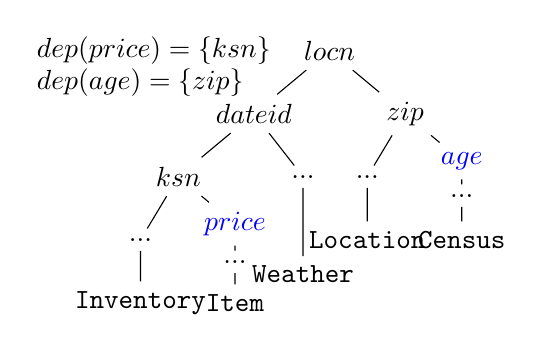
\begin{tikzpicture}[xscale=0.96, yscale=0.8]
  \node at (0, 0) (locn) {$locn$};      
  \node at (-1, -1) (dateid) {$dateid$} edge[-] (locn);
  \node at (-2, -2) (ksn) {$ksn$} edge[-] (dateid);
  \node at (-1.25, -2.75) (subcategory) {$\color{blue} price$} edge[-] (ksn);
  \node at (-1.25, -3.35) (item_p) {...} edge[-] (subcategory);
  \node at (-1.25, -4) (item) {\tt{Item}} edge[-] (item_p);
  \node at (-2.5, -3) (inventoryunits) {...} edge[-] (ksn);
  \node at (-2.5, -4) (inventory) {\tt{Inventory}} edge[-] (inventoryunits);

  \node at (-0.35, -2) (rain) {...} edge[-] (dateid);
  \node at (-0.35, -3.55) (weather) {\tt{Weather}} edge[-] (rain);

  \node at (1, -1) (zip) {$zip$} edge[-] (locn);
  \node at (1.75, -1.75) (population) {$\color{blue} age$} edge[-] (zip);
  \node at (1.75, -2.3) (census_p) {...} edge[-] (population);
  \node at (1.75, -3) (census) {\tt{Census}} edge[-] (census_p);

  \node at (0.5, -2) (rgn_cd) {...} edge[-] (zip);
  \node at (0.5, -3) (location) {\tt{Location}} edge[-] (rgn_cd);

  % dep sets
  \node[anchor=west] at (-4, -0.0) () {$dep(price) = \{ksn\}$};
  \node[anchor=west] at (-4, -0.5) () {$dep(age) = \{zip\}$};
  % \node[anchor=west] at (-4, -1) () {$dep(subcategory) = \{ksn\}$};

  % \node[anchor=west] at (2, 0) () {$dep(locn) = \emptyset$}; 
  % \node[anchor=west] at (2, -.5) () {$dep(zip) = \{locn\}$};
  % \node[anchor=west] at (2, -1.0) () {$dep(population) = \{zip\}$};

\end{tikzpicture} 
}   
\end{minipage} 
\caption{Variable orders for the $q$-hierarchical queries over the {\em Housing} dataset (left), {\em Retailer} dataset (middle) and {\em Favorita} dataset (right). All non-join variables except the blue ones are omitted. The blue variables are the only variables whose dependency sets are not their ancestors.}
\label{fig:q-hierarchical-vos}
\end{figure*}
}

\add{

\subsection{Maintenance of Sum Aggregates}
\label{sec:sum_aggregate_maintenance}

We analyze different strategies for maintaining a sum of one variable on top of a natural join. We measure the average throughput of reevaluation and incremental maintenance under updates of size $1,000$ to all the relations of {\em Retailer} and {\em Housing}. For the former dataset, we sum the inventory units for products in {\tt Inventory}; for the latter, we sum over the common join variable. We also benchmark two reevaluation strategies that recompute the results from scratch on every update: \DFRE denotes reevaluation using variable orders and \DBTRE denotes reevaluation using DBToaster. Table~\ref{table:sum_aggregate_cost_comparison} summarizes the results. 
  

\DF achieves the highest average throughput in both cases. For {\em Retailer}, the maintenance cost is dominated by the update on {\tt Inventory}. 
\DBT's recursive delta compilation materializes $13$ views representing connected subqueries: five group-by aggregates over the input relations, {\tt Inv}, {\tt It}, {\tt W}, {\tt L}, and {\tt C}; one group-by aggregate joining {\tt L} and {\tt C}; six views joining {\tt Inv} with subsets of the others, namely \{{\tt It}\}, \{{\tt It}, {\tt W}\}, \{{\tt It}, {\tt W}, {\tt L}\}, \{{\tt W}\}, \{{\tt W}, {\tt L}\}, and \{{\tt W}, {\tt L}, {\tt C}\}; and the final aggregate.
The two views joining {\tt Inv} with \{ {\tt W}, {\tt L} \} and \{ {\tt It}, {\tt W}, {\tt L} \} require linear maintenance for a single-tuple change in {\tt Inventory}.
\IVM recomputes deltas from scratch on each update using only the input relations with no aggregates on top of them. Updates to {\tt Inventory} are efficient due to small sizes of the other relations. 
\DF uses the given variable order to materialize $9$ views, four of them over {\tt Inventory}, \{{\tt Inv}\}, \{{\tt Inv}, {\tt It}\}, \{ {\tt Inv}, {\tt It}, {\tt W} \}, and the final sum, but each with constant maintenance for single-tuple updates to this relation.
In contrast to \IVM, our approach materializes precomputed views in which all nonjoin variables are aggregated away. 
In the {\em Housing} schema, both \DF and \DBT benefit from this preaggregation, and since the query is a star join, both materialize the same views. \DBT computes {\tt SUM(1)} and {\tt SUM(postcode)} for each {\tt postcode} in the delta for {\tt Inventory}, although only the count suffices.
Figure~\ref{table:sum_aggregate_cost_comparison} also shows that the reevaluation strategies significantly underperform the incremental approaches.


\begin{figure}[t]
\begin{center}
{
\renewcommand{\arraystretch}{1.3}
\begin{small}
\begin{tabular}{@{}l@{~}c@{~}c@{~}c@{~}c@{~}c@{}}
\toprule
  & \DF &  \DBT & \IVM & \DFRE & \DBTRE \\
% \cmidrule{2-4} \cmidrule{6-7} 
\midrule
Retailer \quad & $2,955,045$ &  $1,250,262$ & $2,925,828$ & $3,785^{*}$ & $3,491^{*}$ \\
Housing  \quad & $22,857,143$ & $17,834,395$ & $2,403,433$ & $79,226$ & $364^{*}$ \\
\bottomrule
\end{tabular}
\end{small}
}
\end{center}
\caption{The average throughput (tuples/sec) of reevaluation and incremental maintenance of a sum aggregate under updates of size $1,000$ to all relations of the {\em Retailer} and {\em Housing} datasets with a one-hour timeout (denoted by the symbol$^{*}$).}
\label{table:sum_aggregate_cost_comparison}
% \vspace*{-1.5em}
\end{figure}


%%%%%%%%%%%%%%%%%%%%%%%%%%%%%%%%%



\subsection{Matrix Chain Multiplication}
\label{sec:matrix_chain_multiplication}

\begin{figure*}[t]
  \centering   
  \includegraphics[width=0.47\textwidth]{Figure_MCM1}
  \qquad
  \includegraphics[width=0.47\textwidth]{Figure_MCM2}
  % \vspace*{-1em}
  \caption{Incremental maintenance and reevaluation of the product of three $(n \times n)$ matrices, $A = A_1 \, A_2 \, A_3$: (left) one-row updates in $A_2$; (right) rank-$r$ updates in $A_2$ for $n=4,096$ using the DBToaster and Octave runtime environments. }
  \label{fig:MCM}
\end{figure*}


We consider the problem of maintaining the multiplication $A = A_1 \, A_2 \, A_3$ of three $(n \times n)$ matrices under changes to $A_2$. We compare \DF with factorized updates, \IVM that recomputes the delta $\delta{A} = A_1 \, \delta{A_2} 
\, A_3$ from scratch, and REEVAL that recomputes the entire product from scratch on every update. 
\DBT becomes \IVM in this particular setting.
We consider two different implementations of these maintenance strategies: The first uses DBToaster's hash maps to store matrices, while the second uses Octave, a numerical tool that stores matrices in dense arrays and offers highly-optimized BLAS routines for matrix multiplication~\cite{Whaley1999}. In both cases, matrix-matrix multiplication takes $\bigO{n^{\alpha}}$ for $\alpha > 2$; for instance, $\alpha = 2.8074$ for 
Strassen's algorithm.




We first consider updates to one row in $A_2$. For \IVM, the delta $\delta{A_{12}} = A_1 \, \delta{A_2}$ might  contain non-zero changes to all $n^2$ matrix entries, thus computing $\delta{A} = \delta{A_{12}} \, A_3$ requires full matrix-matrix multiplication. REEVAL updates $A_2$ first before computing two matrix-matrix multiplications. \DF factorizes $\delta{A_2}$ into a product of two vectors $\delta{A_2} = u \TR{v}$, which are used to compute $\delta{A_{12}} = (A_1 \, u) \, \TR{v} = u_1 \, \TR{v}$ and $\delta{A} = u_1 \, (\TR{v} \, A_3) = u_1 \, v_1$. Both deltas involve only matrix-vector multiplications computed in $\bigO{n^2}$ time. 
Figure~\ref{fig:MCM} (left) shows the average time needed to process an update to one randomly selected row in $A_2$ for different matrix sizes. REEVAL performs two matrix-matrix multiplications, while \IVM performs only one. In the hash-based implementation, the gap between \DF and \IVM grows from $28$x for $n=256$ to $92$x for $n=4,096$; similarly, in the Octave implementation, the same gap grows from $16$x for $n=256$ to $236$x for $n=16,384$. This confirms the difference in the asymptotic complexity of these strategies.

Our next experiment considers rank-$r$ updates to $A_2$, which can be decomposed into a sum of $r$ rank-$1$ tensors, $\delta{A_2} = \sum_{i\in[r]} u_i \TR{v_i}$. \DF processes $\delta{A_2}$ as a sequence of $r$ rank-$1$ updates in $\bigO{rn^2}$ time, while both REEVAL and \IVM take as input one full matrix $\delta{A_2}$ and maintain the product in $\bigO{n^3}$ time per each rank-$r$ update. \IVM has the same performance as REEVAL. Figure~\ref{fig:MCM} (right) shows that the average time \DF takes to process a rank-$r$ update for different $r$ values and the matrix size $4,096$ is linear in the tensor rank $r$. 
Under both implementations in DBToaster and Octave, incremental computation is faster than reevaluation for updates with rank $r\leq 96$.
With larger matrix sizes, the gap between reevaluation and incremental computation increases, which enables incremental maintenance for updates of higher ranks.


%%%%%%%%%%%%%%%%%%%%%%%%%%%%%%%%%
\begin{figure*}[t]
  \centering   
  \includegraphics[width=0.48\textwidth]{Figure_FullJoin_Retailer}
  \quad
  \includegraphics[width=0.48\textwidth]{Figure_FullJoin_Housing}
  % \vspace*{-1em}
  \caption{Incremental maintenance using relational and factorized payloads for the natural joins of the {\em Retailer}  (left) and of the {\em Housing} (right) datasets under updates of size $1,000$ to the largest relation ({\em Retailer}) and all input relations ({\em Housing}).}
  \label{fig:FullJoin_Factorized_Relational}
\end{figure*}

\subsection{Factorized Computation of Conjunctive Queries}
\label{sec:factorized_conjunctive}

We analyze \DF on queries whose results are stored as keys with integer multiplicities using listing representation ({\tt List$\;$keys}) and as relational payloads using factorized and listing representations ({\tt Fact$\;$payloads} and {\tt List$\;$payloads}).
Figure~\ref{fig:FullJoin_Factorized_Relational} (left) considers the natural join of {\em Retailer} under updates to the largest relation. The factorized payloads reduce the memory consumption by $4.4$x, from $34$GB to $7.8$GB, improve the average throughput by $2.8$x and $3.7$x (and the overall run time by $3.2$x and $4.2$x) compared to using the two listing encodings.
Figure~\ref{fig:FullJoin_Factorized_Relational} (right) considers the natural join of {\em Housing} under updates to all input relations.  The number of tuples in the dataset varies from $150,000$ (scale 1) to $1,400,000$ (scale 20), while the size of the listing (factorized) representation of natural join grows cubically (linearly) with the scale factor. The two listing encodings blow up the memory consumption and computation time for large scales. Storing tuples in the listing representation using payloads instead of keys avoids the need for hashing wide keys, which makes the joins slightly cheaper. For {\em Housing} and factorized representation, the root view stores $25,000$ values of the join variable regardless of the scale. The root's children map these values to relational payloads for each relation. For the largest scale, {\tt Fact$\;$payloads} is $481$x faster and takes $548$x less memory than {\tt List$\;$payloads} ($410$ms vs. $197$s, $195$MB vs. $104$GB), and {\tt List$\;$keys} exceeds the available memory.



}
